% ------------------------------------------------------------------------------
% TYPO3 Version 10.3 - What's New (French Version)
%
% @license	Creative Commons BY-NC-SA 3.0
% @link		https://typo3.org/help/documentation/whats-new/
% @language	French
% ------------------------------------------------------------------------------

\section{Changements pour les intégrateurs}
\begin{frame}[fragile]
	\frametitle{Changements pour les intégrateurs}

	\begin{center}\huge{Chapitre 2~:}\end{center}
	\begin{center}\huge{\color{typo3darkgrey}\textbf{Changements pour les intégrateurs}}\end{center}

\end{frame}

% ------------------------------------------------------------------------------
% Feature | 90333 | Dashboard

\begin{frame}[fragile]
	\frametitle{Changements pour les intégrateurs}
	\framesubtitle{Tableau de bord}

	% decrease font size for code listing
	\lstset{basicstyle=\tiny\ttfamily}

	\begin{itemize}
		\item Il est possible de définir des \textit{prédéfinitions} de tableau de bord
			pour les nouveaux utilisateurs et ceux qui ont supprimé le leur.
		\item Ceci permet d'afficher tableau de bord «~Pour débuter~» par défaut.
		\item Exemple de TSconfig~:

\vspace{-0.4cm}
\begin{lstlisting}
options.dashboard.dashboardPresetsForNewUsers = default, dashboardPreset-myPreset
\end{lstlisting}

		\item De multiples prédéfinitions de tableau de bord peuvent être définis sous
			forme de liste à virgule.

	\end{itemize}

\end{frame}

% ------------------------------------------------------------------------------
% Important | 89992 | Use New TranslationServer

\begin{frame}[fragile]
	\frametitle{Changements pour les intégrateurs}
	\framesubtitle{Plateforme de gestion des traductions}

	\begin{itemize}
		\item La solution SaaS \href{https://crowdin.com/}{Crowdin} est maintenant la
			plateforme de gestion des traductions pour TYPO3.
		\item Nous encourageons tous les monde à participer et améliorer la traduction.
		\item Crowdin est utilisé pour traduire les libellés de langue du noyau de TYPO3
			ainsi que ceux des extensions TYPO3.
		\item En savoir plus dans la
			\href{https://docs.typo3.org/m/typo3/reference-coreapi/master/en-us/ApiOverview/Internationalization/TranslationServer/Crowdin.html}{documentation TYPO3}.
	\end{itemize}

	\begin{figure}
		
\includegraphics[width=0.40\linewidth]{ChangesForIntegrators/crowdin-logo.png}
	\end{figure}

\end{frame}

% ------------------------------------------------------------------------------
% Feature | 90266 | Fluid-based templated emails

\begin{frame}[fragile]
	\frametitle{Changements pour les intégrateurs}
	\framesubtitle{Emails HTML basés sur Fluid (1)}

	% decrease font size for code listing
	\lstset{basicstyle=\smaller\ttfamily}

	\begin{itemize}
		\item Les contenus des emails HTML et texte brute sont basés sur des templates.
		\item Ils sont générés à l'aide du moteur de rendu Fluid.
		\item La personnalisation s'effectue en surchargeant les chemins vers les fichiers~:

\vspace{-0.4cm}
\begin{lstlisting}
$GLOBALS['TYPO3_CONF_VARS']['MAIL']['templateRootPaths'][700] =
  'EXT:my_site_extension/Resources/Private/Templates/Email';

$GLOBALS['TYPO3_CONF_VARS']['MAIL']['layoutRootPaths'][700] =
  'EXT:my_site_extension/Resources/Private/Layouts';
\end{lstlisting}

	\end{itemize}

\end{frame}

% ------------------------------------------------------------------------------
% Feature | 90266 | Fluid-based templated emails

\begin{frame}[fragile]
	\frametitle{Changements pour les intégrateurs}
	\framesubtitle{Emails HTML basés sur Fluid (2)}

	\begin{itemize}
		\item Par exemple, les composants suivants utilisent les templates Fluid~:

			\begin{itemize}
				\item Message de test de l'outil d'installation (voir l'exemple sur la prochaine diapositive).
				\item Messages de notification des espaces de travail lors du changement d'étape.
				\item Message de notification de connexion d'un utilisateur backend.
			\end{itemize}

	\end{itemize}

\end{frame}

% ------------------------------------------------------------------------------
% Feature | 90266 | Fluid-based templated emails

\begin{frame}[fragile]
	\frametitle{Changements pour les intégrateurs}
	\framesubtitle{Emails HTML basés sur Fluid (3)}

	Message de test envoyé depuis l'outil d'installation~:

	\begin{figure}
		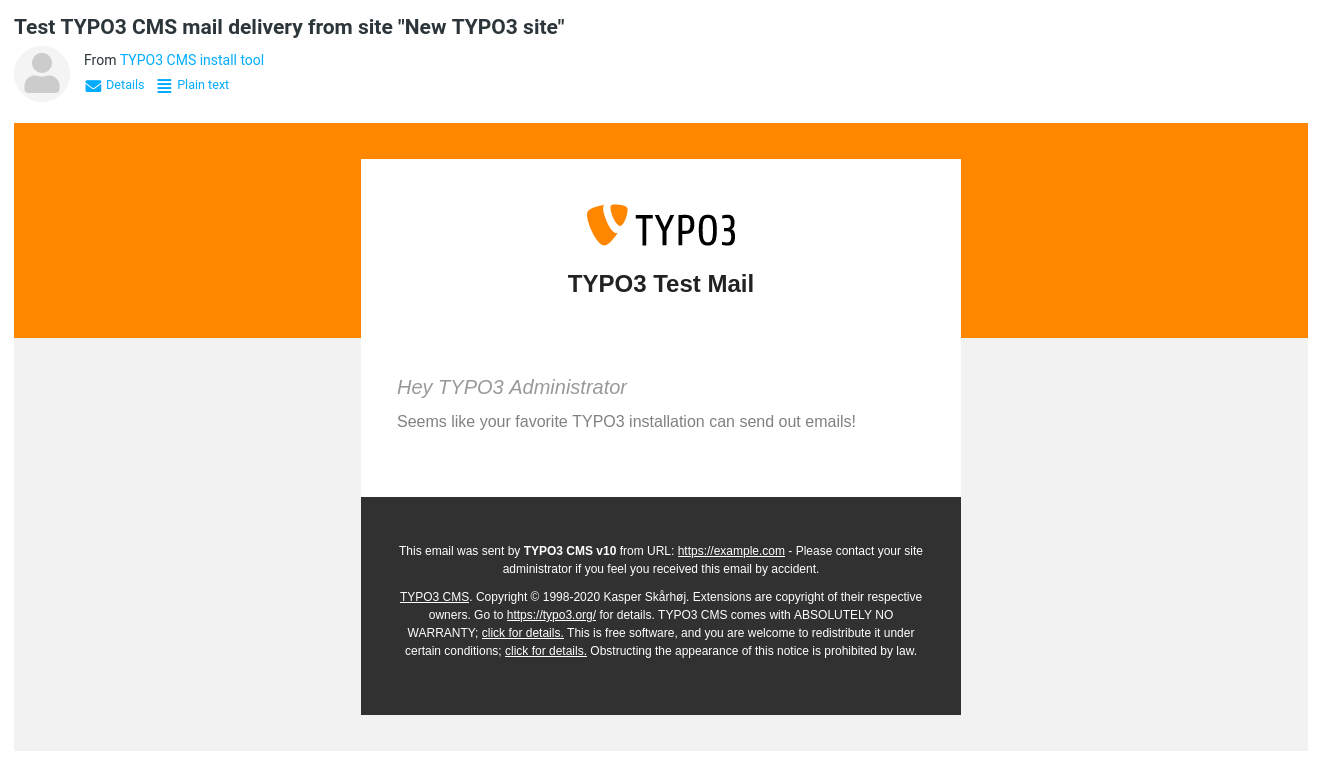
\includegraphics[width=0.8\linewidth]{ChangesForIntegrators/90266-FluidBasedTemplatedEmails.png}
	\end{figure}

\end{frame}

% ------------------------------------------------------------------------------
% Feature | 90203 | Make workspace available in TypoScript conditions

\begin{frame}[fragile]
	\frametitle{Changements pour les intégrateurs}
	\framesubtitle{Espaces de travail et TypoScript}

	% decrease font size for code listing
	\lstset{basicstyle=\smaller\ttfamily}

	\begin{itemize}
		\item La variable \texttt{workspace} est introduite dans le langage des expressions.
		\item Cette variable est utilisée pour faire correspondre l'expression avec les
			paramètres communs des espaces de travail.
		\item Actuellement, ces paramètres sont supportés~:\newline
			\small
				\texttt{workspaceId}, \texttt{isLive}, et \texttt{isOffline}.
			\normalsize
		\item Par exemple~:

\vspace{-0.4cm}
\begin{lstlisting}
[workspace.workspaceId === 3]
  # Current workspace ID is 3
[end]
\end{lstlisting}

	\end{itemize}

\end{frame}

% ------------------------------------------------------------------------------
% Feature | 88962 | Re-implement old PIDupinRootline TypoScript condition

\begin{frame}[fragile]
	\frametitle{Changements pour les intégrateurs}
	\framesubtitle{TypoScript}

	% decrease font size for code listing
	\lstset{basicstyle=\smaller\ttfamily}

	\begin{itemize}
		\item L'ancienne condition \texttt{PIDupinRootline} est réimplémenté
			en TypoScript dans le langage d'expression de Symfony.
		\item Ancienne syntaxe de la condition TypoScript~:

\vspace{-0.4cm}
\begin{lstlisting}
[PIDupinRootline = 30]
  page.10.value = I'm on any subpage of page with UID 30.
[END]
\end{lstlisting}

		\item Nouvelle syntaxe de la condition TypoScript~:

\vspace{-0.4cm}
\begin{lstlisting}
[30 in tree.rootLineParentIds]
  page.10.value = I'm on any subpage of page with UID 30.
[END]
\end{lstlisting}

	\end{itemize}

\end{frame}

% ------------------------------------------------------------------------------
% Feature | 90426 | Browser-native lazy loading for images

\begin{frame}[fragile]
	\frametitle{Changements pour les intégrateurs}
	\framesubtitle{Chargement différé des images}

	% decrease font size for code listing
	\lstset{basicstyle=\smaller\ttfamily}

	\begin{itemize}
		\item L'attribut HTML \texttt{loading} est disponible pour les balises \texttt{<img>}.
		\item Les navigateurs supportant cette fonctionnalité ne chargeront pas ces images
			avant qu'elles soient visibles.
		\item Le comportement est modifiable avec la constante TypoScript suivante~:

\vspace{-0.4cm}
\begin{lstlisting}
styles.content.image.lazyLoading = lazy
\end{lstlisting}

		\item Les valeurs valides sont~: \texttt{lazy} (default), \texttt{eager}, et \texttt{auto}.
		\item Le ViewHelper Fluid \textit{Image} supporte aussi cet attribut~:

\vspace{-0.4cm}
\begin{lstlisting}
<f:image src="{fileObject}" treatIdAsReference="true"
  loading="lazy" />
\end{lstlisting}

	\end{itemize}

\end{frame}

% ------------------------------------------------------------------------------
% Important | 89869 | Change lockIP default to disabled for both frontend and backend

\begin{frame}[fragile]
	\frametitle{Changements pour les intégrateurs}
	\framesubtitle{Valeurs par défaut pour \texttt{lockIP}/\texttt{lockIPv6}}

	% decrease font size for code listing
	\lstset{basicstyle=\smaller\ttfamily}

	\begin{itemize}
		\item Les valeurs par défaut pour les options \texttt{lockIP} ont changées.
		\item Ces quatre variables système suivantes sont \textbf{désactivées} par défaut~:

			\begin{itemize}
				\item \texttt{[FE]['lockIP']}
				\item \texttt{[FE]['lockIPv6']}
				\item \texttt{[BE]['lockIP']}
				\item \texttt{[BE]['lockIPv6']}
			\end{itemize}

		\item Les anciennes valeur par défaut (\texttt{4} pour le backend et \texttt{2} pour le frontend)
			posaient des problèmes pour les clients supportant IPv4 et IPv6.

	\end{itemize}

\end{frame}

% ------------------------------------------------------------------------------
% Feature | 90052 | Form YAML configuration available in configuration module

\begin{frame}[fragile]
	\frametitle{Changements pour les intégrateurs}
	\framesubtitle{Formulaires~: Configuration YAML}

	\begin{columns}[T]
		\begin{column}{.04\textwidth}
		\end{column}
		\begin{column}{.38\textwidth}

			Lorsque l'extension système \texttt{EXT:form} est activée, la configuration YAML chargée
			est disponible sous \textbf{SYSTÈME} $\rightarrow$ \textbf{Configuration}.

			\vspace{0.2cm}

			Ceci nécessite bien sûr que l'extension \texttt{EXT:lowlevel} soit activée.

		\end{column}
		\begin{column}{.58\textwidth}
			\vspace{-0.3cm}
			\begin{figure}
				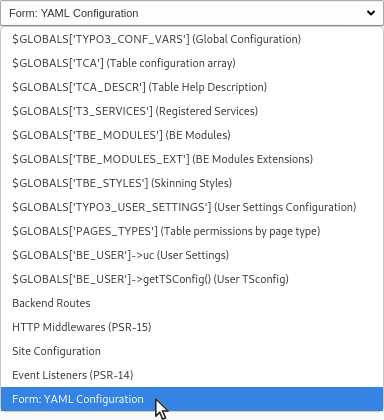
\includegraphics[width=0.70\linewidth]{ChangesForIntegrators/90052-AddYamlConfigurationToConfigurationModule.png}
			\end{figure}
		\end{column}
	\end{columns}

\end{frame}

% ------------------------------------------------------------------------------
% Feature | 88147 | Add possibility to configure the path to sitemap xslFile

\begin{frame}[fragile]
	\frametitle{Changements pour les intégrateurs}
	\framesubtitle{SEO~: \texttt{Sitemap.xsl}}

	% decrease font size for code listing
	\lstset{basicstyle=\tiny\ttfamily}

	\begin{itemize}
		\item Le chemin par défaut du fichier \texttt{Sitemap.xsl} de l'extension
			système \texttt{EXT:seo} est modifiable~:

\vspace{-0.4cm}
\begin{lstlisting}
# Globally for all sitemaps:
plugin.tx_seo.config.xslFile = EXT:myext/Resources/Public/CSS/mySite.xsl

# For all sitemaps of a specific type:
plugin.tx_seo.config.<sitemapType>.sitemaps.xslFile = EXT:myext/Resources/Public/CSS/mySite.xsl

# For a specific sitemap:
plugin.tx_seo.config.<sitemapType>.sitemaps.<sitemap>.config.xslFile =
  EXT:myext/Resources/Public/CSS/mySite.xsl
\end{lstlisting}

		\item Le chemin par défaut est~:\newline
			\smaller
				\texttt{EXT:seo/Resources/Public/CSS/Sitemap.xsl}
			\normalsize

	\end{itemize}

\end{frame}

% ------------------------------------------------------------------------------
% Feature | 82062 | Progress for Reference Index update on CLI

\begin{frame}[fragile]
	\frametitle{Changements pour les intégrateurs}
	\framesubtitle{Index des références}

	% decrease font size for code listing
	\lstset{basicstyle=\tiny\ttfamily}

	\begin{itemize}
		\item Pendant la mise à jour de l'index des références, des barres de progression sont
			affichées pour chaque tables de la base.
	\end{itemize}

	\begin{figure}
		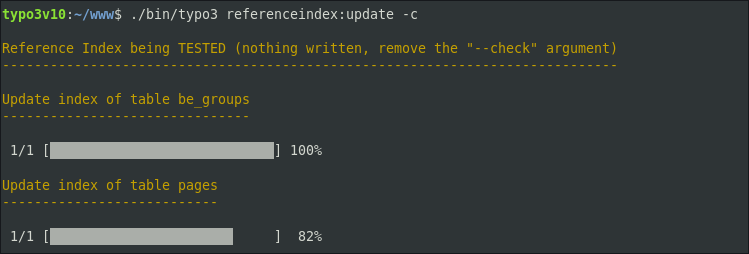
\includegraphics[width=0.85\linewidth]{ChangesForIntegrators/82062-ProgressForReferenceIndexUpdateOnCli.png}
	\end{figure}

\end{frame}

% ------------------------------------------------------------------------------
% Feature | 90425 | Add seo fields to info module

\begin{frame}[fragile]
	\frametitle{Changements pour les intégrateurs}
	\framesubtitle{Module Information}

	\begin{itemize}
		\item Les informations SEO et de média sociaux sont affichées dans le module Information~:\newline
			\textbf{WEB} $\rightarrow$ \textbf{Info} $\rightarrow$ \textbf{Aperçu de l'arborescence}.
	\end{itemize}

	\begin{figure}
		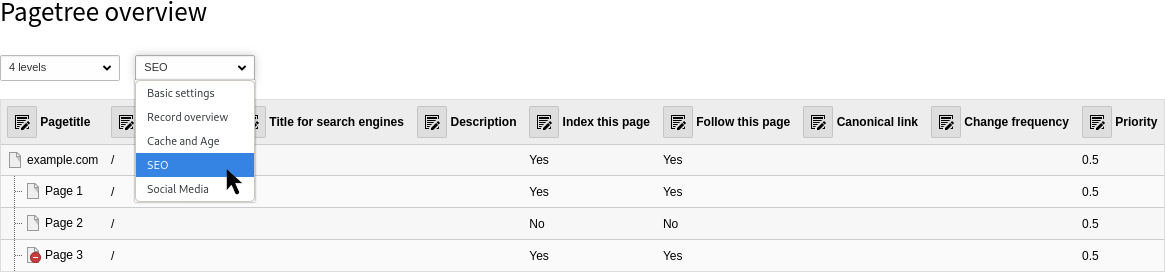
\includegraphics[width=0.85\linewidth]{ChangesForIntegrators/90425-AddSeoFieldsToInfoModule.png}
	\end{figure}

\end{frame}

% ------------------------------------------------------------------------------
% Feature | 59452 | scheduler:run command accepts multiple task options

\begin{frame}[fragile]
	\frametitle{Changements pour les intégrateurs}
	\framesubtitle{Planificateur}

	% decrease font size for code listing
	\lstset{basicstyle=\tiny\ttfamily}

	\begin{itemize}
		\item Il est possible d'exécuter plusieurs tâches lorsque l'option \texttt{-}\texttt{-}\texttt{task} est utilisée
	\end{itemize}

	\begin{figure}
		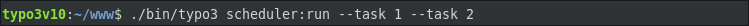
\includegraphics[width=0.85\linewidth]{ChangesForIntegrators/59452a-MultipleTasksInSchedulerCommand.png}
	\end{figure}

	\begin{itemize}
		\item La sortie verbeuse est activée avec \texttt{-}\texttt{v} et \texttt{-}\texttt{vv}
	\end{itemize}

	\begin{figure}
		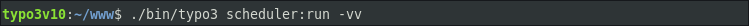
\includegraphics[width=0.85\linewidth]{ChangesForIntegrators/59452b-MultipleTasksInSchedulerCommand.png}
	\end{figure}

\end{frame}

% ------------------------------------------------------------------------------
% Feature | 90298 | Improve user info in BE User module

\begin{frame}[fragile]
	\frametitle{Changements pour les intégrateurs}
	\framesubtitle{Module Utilisateurs backend}

	\begin{itemize}
		\item Une vue détail pour les enregistrement d'utilisateur backend affiche les droits pertinents est ajoutée
		\item Des champs supplémentaires sont ajoutés à la fonction de comparaison des utilisateurs.
		\item Cette fonction prend en compte les sous-groupes.
		\item L'interface utilisateur du module sera encore ajusté et optimisé.
		\item Ces changements facilitent la vérification et la comparaison des permissions des
			utilisateur sans changer d'utilisateur par les intégrateurs/administrateurs.
	\end{itemize}

\end{frame}

% ------------------------------------------------------------------------------
% Feature | 89894 | Separate system extensions from 3rd-party extensions visually

\begin{frame}[fragile]
	\frametitle{Changements pour les intégrateurs}
	\framesubtitle{Gestionnaire d'extensions}

	Les extensions peuvent être filtrées par système et tierce dans le gestionnaire d'extensions.

	\begin{figure}
		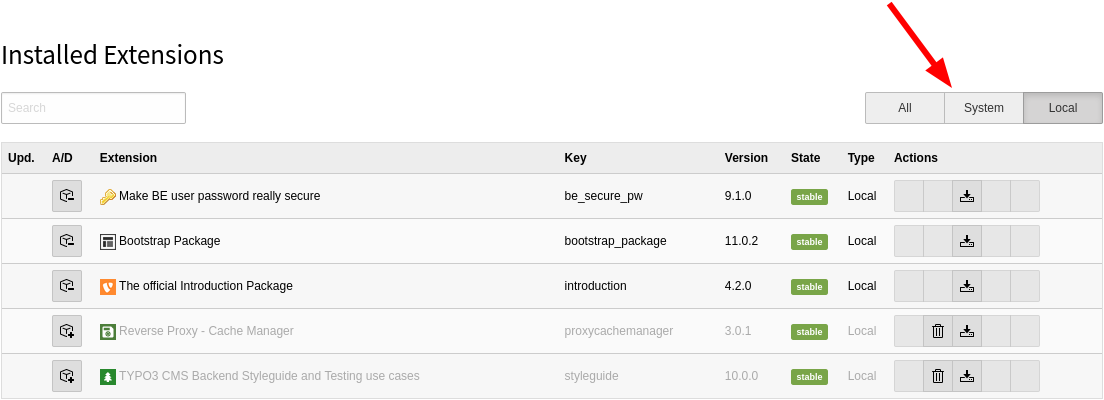
\includegraphics[width=0.9\linewidth]{BackendUserInterface/89894-SeparateSystemExtensionsFrom3rdPartyExtensionsVisually.png}
	\end{figure}

\end{frame}

% ------------------------------------------------------------------------------
% Feature | 90136 | Show application context in the Environment module

\begin{frame}[fragile]
	\frametitle{Changements pour les intégrateurs}
	\framesubtitle{Aperçu de l'environnement}

	Le contexte d'application actuel est affiché dans le module Environnement~:\newline
	\textbf{OUTILS D'ADMINISTRATION} $\rightarrow$ \textbf{Environnement} $\rightarrow$ \textbf{Aperçu de l'environnement}.

	\begin{figure}
		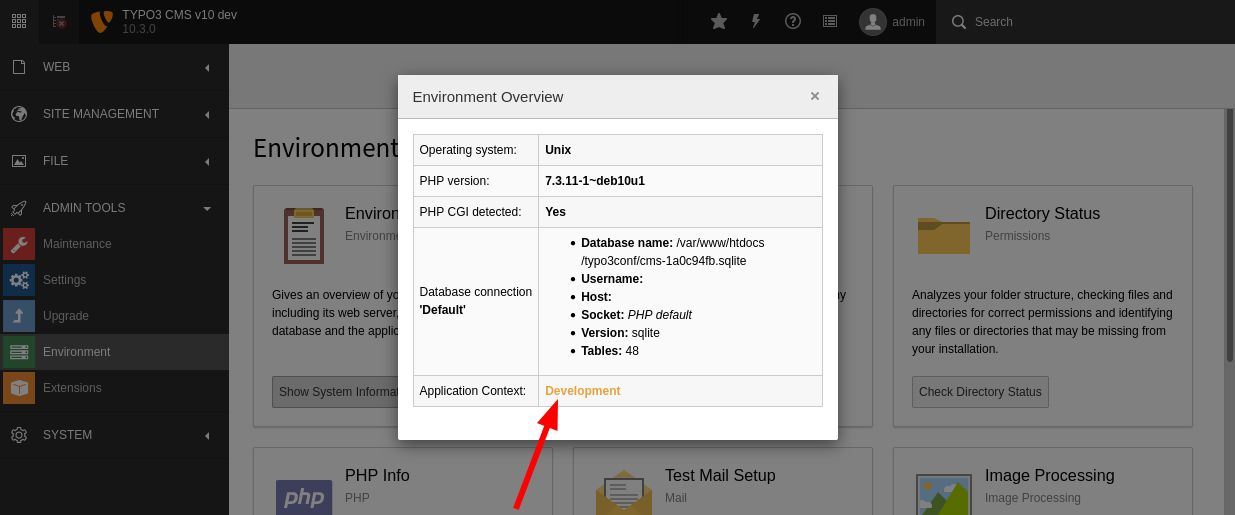
\includegraphics[width=0.9\linewidth]{ChangesForIntegrators/90136-ShowApplicationContextInTheEnvironmentModule.png}
	\end{figure}

\end{frame}

% ------------------------------------------------------------------------------
% Task | 89844 | Improve visual appearance of feature toggles

\begin{frame}[fragile]
	\frametitle{Changements pour les intégrateurs}
	\framesubtitle{Configuration des fonctionnalités}

	L'apparence visuelle des bascules de fonctionnalité est améliorée~:
	\newline\newline
	\smaller\textbf{TYPO3 < 10.3}\tabto{6cm}\textbf{TYPO3 >= 10.3}\normalsize

	\begin{figure}
		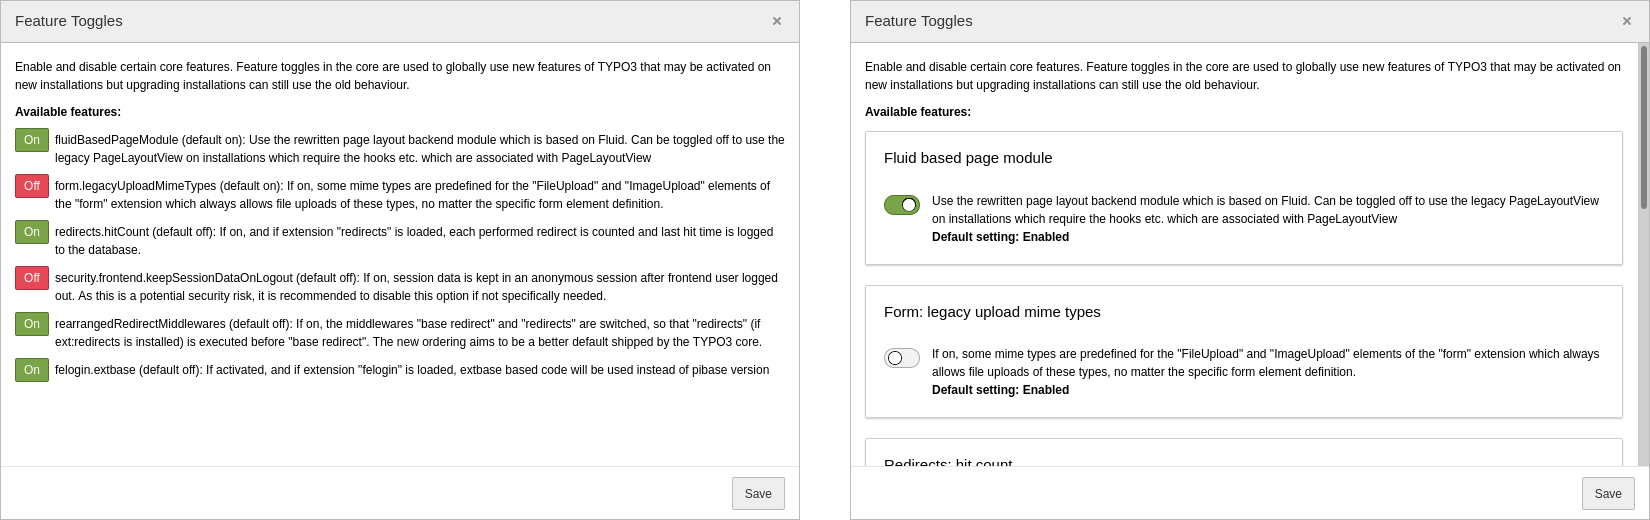
\includegraphics[width=1\linewidth]{ChangesForIntegrators/89844-ImproveVisualAppearanceOfFeatureToggles.png}
	\end{figure}

\end{frame}

% ------------------------------------------------------------------------------
% Feature | 89513 | Provide password recovery for backend users
%
%\begin{frame}[fragile]
%	\frametitle{Changements pour les intégrateurs}
%	\framesubtitle{Message de récupération de mot de passe}
%
%	\begin{itemize}
%
%		\item Les liens de réinitialisation de mots de passe ne sont valides que pour 4 heures.\newline
%			Cette limite n'est pas configurable.
%		\item La fonction est désactivable pour tous les utilisateurs ou seulement les administrateurs pour renforcer la sécurité.
%		\item Si des utilisateurs partagent une adresse, un texte alternatif de message est utilisé.
%		\item Le champ TCA \texttt{be\_users.email} ne doit pas avoir \texttt{eval=email} de défini.
%
%		\item La fonction ne s'applique que pour les utilisateurs qui~:
%			\begin{itemize}
%				\item ont une adresse email de définie,
%				\item ont un mot de passe de défini, et
%				\item ne sont pas désactivé/supprimé.
%			\end{itemize}
%
%	\end{itemize}
%
%\end{frame}
%
% ------------------------------------------------------------------------------
